\chapter{Methodology}\label{ch:methods}
The methods described in this chapter are adapted from the ideas discussed in \cite[Section 4]{cg_sharpened_convrate_Axelsson1976}. Therein \citeauthor{cg_sharpened_convrate_Axelsson1976} presents a sharpened CG iteration bound for two characteristic eigenspectra. The eigenspectrum consisting of two disjoint clusters and the \textit{two-cluster} bound $m_2$ developed for it in \cref{sec:cg_sharpened_convrate} are central to this thesis. Alongside the treatment of the two-cluster eigenspectrum is the analysis of the related \textit{tail-cluster} eigenspectrum. Remarkably, the CG iteration bound for the tail-cluster eigenspectrum is also contained within the bound $m_2$. In \cref{sec:performance_ratio} the two-cluster bound is compared to its classical predecessor $m_1$ from \cref{eq:cg_convergence_rate_bound_iterations_approx}, where a necessary condition is derived for which $m_2 < m_1$. Similarly, in \cref{sec:tail_cluster_bound_performance} the tail-cluster variant of $m_2$ is compared to $m_1$, resulting in another necessary condition for $m_2 < m_1$. The two-cluster bound is then generalized to a multiple-tail-cluster bound in \cref{sec:multiple_clusters}. Finally, in \cref{sec:cg_iteration_bound_algorithm} the conditions obtained in \cref{sec:performance_ratio,sec:tail_cluster_bound_performance} and the generalized multiple-tail-cluster bound are combined with an eigenspectrum partitioning algorithm culminating in \cref{alg:multi_cluster_cg_bound,alg:multi_tail_cluster_cg_bound}, yielding two novel and sharpened CG iteration bounds.

\section{Two cluster case}\label{sec:cg_sharpened_convrate}
On the eigenspectrum of $A$, consider two intervals $[a, b]$ and $[c, d]$ with $0 < a < b < c < d$ such that all eigenvalues of $A$ are contained in the union of these two intervals. Additionally, we have $\kappa(A) = \frac{d}{a}$. We treat the following two cases simultaneously
\begin{equation}
    \sigma_1(A) = [a,b] \bigcup [c,d]
    \label{eq:two_clusters}
\end{equation}
\begin{equation}
    \sigma_2(A) = [c,d] \bigcup_{\substack{i=1 \\ \lambda_i \in [a,b]}}^{N_{\text{tail}}} \lambda_i
    \label{eq:one_cluster_with_tail}
\end{equation}
where $N_{\text{tail}}$ is the number of eigenvalues in the tail. The first case is a two-cluster eigenspectrum, while the second case has one cluster and a tail of eigenvalues. These characteristic eigenspectra are illustrated in \cref{fig:eigenvalue_clusters}.
\begin{figure}[H]
    \centering
    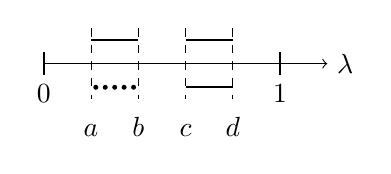
\begin{tikzpicture}[scale=3]

    % Axis
    \draw[->] (0,0) -- (1.2,0) node[right] {$\lambda$};

    % Tick marks and labels at 0 and 1
    \foreach \x/\label in {0/0, 1/1}
    {
        \draw[thick] (\x,0.05) -- (\x,-0.05);
        \node[below=4pt] at (\x,0) {$\label$};
    }

    % Two disjoint clusters
    \draw[thick] (0.2,0.1) -- (0.4,0.1);
    \draw[thick] (0.6,0.1) -- (0.8,0.1);
    % \node[above] at (0.3,0.1) {Cluster 1};
    % \node[above] at (0.7,0.1) {Cluster 2};
    % \node[left] at (0,0.1) {\small Two disjoint clusters};
    
    % Cluster with tail
    \draw[thick] (0.6,-0.1) -- (0.8,-0.1); % main cluster
    \foreach \x in {0.22,0.26,0.30,0.34,0.38} 
        \fill (\x,-0.1) circle (0.3pt); % tail eigenvalues
    % \node[below] at (0.7,-0.1) {Main cluster};
    % \node[below] at (0.3,-0.1) {Tail};
    % \node[left] at (0,-0.1) {\small Cluster with tail};
    
    % Mark points a, b, c, d
    \foreach \x/\label in {0.2/a, 0.4/b, 0.6/c, 0.8/d}
    {
        \draw[thin,dashed] (\x,0.15) -- (\x,-0.15);
        \node[above] at (\x,-0.35) {$\label$};
    }
    
\end{tikzpicture}
    \caption{Eigenspectrum of $A$ with two clusters (above) and a combination of a tail and cluster (below).}
    \label{fig:eigenvalue_clusters}
\end{figure}

The CG error \cref{eq:cg_error_bound} suggests we look for a polynomial $r_{m_2}$ of degree $m_2$ that satisfies the constraints of the minimization problem in order to find an iteration bound $m < m_2$. In other words, we do not solve the minimization problem directly, but we make a clever selection of the polynomial $r_{m_2}$ that satisfies the constraints. As a consequence, the actual minimizing polynomial might require a lower degree $m$ to satisfy the same relative error tolerance $\epsilon$. Therefore, the degree $m_2$ we find is at least as large as the actual number of iterations required to achieve the desired relative error tolerance $\epsilon$.

\citeauthor{cg_sharpened_convrate_Axelsson1976} suggests we use not one monolithic residual polynomial function, but a multiplication of two residual polynomial functions $\hat{r}^{(i)}_p(x)$ and $\hat{r}_{m_2-p}(x)$ for the two clusters. The superscript $^{(i)}$ corresponds to the two eigenspectra described above. The residual polynomial functions are defined using \cref{def:scaled_chebyshev_polynomial} and $\gamma = 0$ as follows
\begin{equation}
    \hat{r}^{(i)}_p (x)
    \begin{cases}
        \hat{C}_p                                            & , \text{if } i = 1                      \\
        \overset{p}{\underset{j=1}{\prod}} (1 - x/\lambda_j) & , \text{if } i = 2, p = N_{\text{tail}} \\
    \end{cases}
    \label{eq:residual_polynomial_rm}
\end{equation}
and
\begin{equation}
    \hat{r}_{{m_2}-p} (x) = \frac{C_{m_2-p} \left(\frac{d + c - 2x}{d - c}\right)}{C_{m_2-p}\left(\frac{d + c}{d - c}\right)},
    \label{eq:residual_polynomial_rpm}
\end{equation}
Indeed, the product $r_{m_2} = \hat{r}_p \hat{r}_{m_2-p} \in \mathcal{P}_{m_2}$. Hence, we can use the residual polynomial functions to bound the error at the $m^{\text{th}}$ iterate. Now, we obtain the following intermediate bounds
\begin{subequations}
    \begin{align}
        \max_{\lambda \in [a,b]} |r_{m_2}(\lambda)| \leq \max_{\lambda \in [a,b]} |\hat{r}^{(i)}_p(\lambda)| \max_{\lambda \in [a,b]} |\hat{r}_{m_2-p}(\lambda)| & \leq \max_{\lambda \in [a,b]} |\hat{r}^{(i)}_p(\lambda)|, \ \text{and} \label{eq:residual_polynomial_bound_ab}                     \\
        \max_{\lambda \in [c,d]} |r_{m_2}(\lambda)| \leq \max_{\lambda \in [c,d]} |\hat{r}^{(i)}_p(\lambda)| \max_{\lambda \in [c,d]} |\hat{r}_{m_2-p}(\lambda)| & \leq \max_{\lambda \in [c,d]} |\hat{r}_{p}(\lambda)|/C_{m_2-p}\left(\frac{d+c}{d-c}\right) \label{eq:residual_polynomial_bound_cd}
    \end{align}
\end{subequations}
where the \cref{eq:residual_polynomial_bound_ab} follows from the fact that $|\hat{r}_{m_2-p}(x)| < 1 \ \forall x \in [a,b]$ and \cref{eq:residual_polynomial_bound_cd} from
\[
    \left|C_{m_2-p}\left(\frac{d+c -2x}{d-c}\right)\right| < 1 \ \forall x \in [c,d].
\]

Furthermore, using \cref{eq:chebyshev_polynomial_approximation}, we have
\begin{equation}
    \frac{1}{C_{k}\left(\frac{z_1 + z_2}{z_1 - z_2}\right)} \leq 2 \left(\frac{\sqrt{z_2} - \sqrt{z_1}}{\sqrt{z_2} + \sqrt{z_1}}\right)^k, \text{ for } z_1 > z_2 > 0 \text{ and } k \in \mathbb{N}^+,
    \label{eq:chebyshev_polynomial_bound}
\end{equation}
and
\begin{equation}
    \max_{\lambda \in [a,b]} |\hat{r}^{(i)}_p(\lambda)| \leq
    \begin{cases}
        2\left(\frac{\sqrt{b}-\sqrt{a}}{\sqrt{b}+\sqrt{a}}\right)^p=\eta_1 & , \text{if } i = 1,                      \\
        \left(\frac{b}{a}-1\right)^p=\eta_2                                & , \text{if } i = 2, p = N_{\text{tail}},
    \end{cases}
    \label{eq:residual_polynomial_bound_ab_i}
\end{equation}
Note that if $i=1$ we can determine $p$ by requiring that the maximum of the residual polynomial function $\hat{r}^{(i)}_p$ in $[a,b]$ is equal to $\epsilon$. This gives the following equation
\begin{equation}
    p \leq \left\lfloor\frac{1}{2}\sqrt{\frac{b}{a}}\ln{\frac{2}{\epsilon}} + 1\right\rfloor
    \label{eq:chebyshev_degree_p}
\end{equation}
Also note that for $i=2$ $\hat{r}^{(2)}_p(\lambda) = 0 < \epsilon$ for all eigenvalues $\lambda \in [a,b]$.

Next, $\hat{r}^{(i)}_p$ in $[c,d]$ is bounded by its maximum value within $[a,b]$ multiplied by the polynomial that is the fastest growing polynomial in $\mathcal{P}_{p}$ outside- and bounded below 1 within $[a,b]$. This polynomial is again the (transformed) Chebyshev polynomial $C_{p}\left(\frac{2x - b - a}{b - a}\right)$. Therefore,
\begin{equation*}
    \max_{\lambda \in [c,d]} |\hat{r}^{(i)}_p(\lambda)| \leq \eta_i C_{p}\left(\frac{2d - b - a}{b + a}\right),
\end{equation*}
with $\eta_i$ as defined in \cref{eq:residual_polynomial_bound_ab_i}.

At this point we have ensured that $\max_{\lambda \in [a,b]}|r_{m_2}|$ is bounded by $\epsilon$ using \cref{eq:residual_polynomial_bound_ab}. So it remains to bound $\max_{\lambda \in [c,d]}|r_{m_2}|$ in \cref{eq:residual_polynomial_bound_cd}. Using above results we can write
\begin{equation*}
    \max_{\lambda \in [c,d]} |r_{m_2}(\lambda)| < \epsilon,
\end{equation*}
if we require that
\begin{equation}
    \eta_i C_{p}\left(\frac{2d - b - a}{b - a}\right) /C_{m_2-p}\left(\frac{d+c}{d-c}\right) < \epsilon.
    \label{eq:relative_error_bound_mp}
\end{equation}
Using that for $x_1, x_2, x_3 \in \mathbb{R}^+$ with $x_1 > x_3$ and $z = \frac{x_1 - x_2}{x_3}$
\begin{align*}
    C_p(z) & \leq \left(z + \sqrt{z^2 - 1}\right)^p                                                    \\
           & = \left( \frac{x_1 - x_2}{x_3} + \sqrt{ \left[\frac{x_1 - x_2}{x_3}\right]^2 -1}\right)^p \\
           & \leq \left( \frac{x_1}{x_3} + \sqrt{ \left[\frac{x_1}{x_3}\right]^2 - 1}\right)^p         \\
           & \leq \left( \frac{2x_1}{x_3}\right)^p,
\end{align*}
and substituting $x_1 = 2d$, $x_2 = b + a$ and $x_3 = b - a$ we obtain the following inequality
\begin{equation}
    \eta_i \left(\frac{4d}{b-a} \right)^p /C_{m_2-p}\left(\frac{d+c}{d-c}\right) < \epsilon.
    \label{eq:chebyshev_degree_p_bound}
\end{equation}
Moreover,
\begin{align*}
    \eta_i \left(\frac{4d}{b-a}\right)^p & =
    \begin{cases}
        2\left(\frac{\sqrt{b} - \sqrt{a}}{\sqrt{b} + \sqrt{a}} \frac{4d}{b-a}\right)^p & , \text{if } i = 1  \\
        \left(\frac{b - a}{a}\frac{4d}{b-a}\right)^p                                   & , \text{if } i = 2,
    \end{cases} \\
                                         & =
    \begin{cases}
        2\left(\frac{4d}{b + 2\sqrt{ab} + a}\right)^p & , \text{if } i = 1  \\
        \left(\frac{4d}{a}\right)^p                   & , \text{if } i = 2,
    \end{cases}                                                                                                                                \\
                                         & \leq 2
    \begin{cases}
        \left(\frac{4d}{b}\right)^p & , \text{if } i = 1  \\
        \left(\frac{4d}{a}\right)^p & , \text{if } i = 2,
    \end{cases}
\end{align*}
We can therefore require that the bound in \cref{eq:chebyshev_degree_p_bound} is satisfied if we have
\[
    1/C_{m_2-p}\left(\frac{d+c}{d-c}\right) \leq \frac{\epsilon}{2\left( \frac{4d}{e_i}\right)^p},
\]
where
\[
    e_i = \begin{cases}
        b & , \text{if } i = 1  \\
        a & , \text{if } i = 2. \\
    \end{cases}
\]
Again using \cref{eq:chebyshev_polynomial_bound} and solving for the degree $m_2 - p$ we obtain
\[
    m_2 - p \leq \frac{1}{2}\sqrt{\frac{d}{c}}\left(\ln\left(\frac{2}{\epsilon}\right) + p \ln\left(\frac{4d}{e_i}\right)\right),
\]
which leads to the following bound for the number of iterations \cite[Equation 4.4]{cg_sharpened_convrate_Axelsson1976}
\begin{equation}
    m_2=\left\lfloor\frac{1}{2} \sqrt{\frac{d}{c}} \ln (2 / \epsilon)+\left(1+\frac{1}{2} \sqrt{\frac{d}{c}} \ln (4 d / e_i)\right) p\right\rfloor,
    \label{eq:cg_iteration_bound_2_clusters}
\end{equation}
where
\[
    1 \leq p \leq \min\left(\left\lfloor\frac{1}{2}\sqrt{\frac{b}{a}}\ln{\frac{2}{\epsilon}} + 1 \right\rfloor, N_{\text{tail}}\right).
\]

\section{Performance ratio of the two-cluster bound}\label{sec:performance_ratio}
In this section we assume that we are dealing with an eigenspectrum of the form $\sigma_1(A)$, i.e. we are only treating case 1. For this case, we compare the new bound in \cref{eq:cg_iteration_bound_2_clusters} to the (approximated) classical bound in \cref{eq:cg_convergence_rate_bound_iterations_approx}. We will see that the new bound is not absolutely sharper than the classical one. However, we will derive an approximate, though accurate, criterion (see \cref{eq:threshold_inequality_explicit_expansion}) that allows us to discern under what conditions the new bound \textit{is} sharper.

To that end, we restate \cref{eq:cg_convergence_rate_bound_iterations_approx} here for easy reference
\[
    m_1(\kappa) = \left\lfloor\frac{\sqrt{\kappa}}{2}\ln\left(\frac{2}{\epsilon}\right) + 1\right\rfloor.
\]
Note that $\epsilon$ is generally a predetermined constant. Therefore, we leave it out as an argument of $m_1$ and $m_2$. We also rewrite the bound from \cref{eq:cg_iteration_bound_2_clusters} in terms of the left and right cluster condition numbers $\kappa_l = \frac{b}{a} > 1$ and $\kappa_r = \frac{d}{b} > 1$ as
\[
    m_2(\kappa, \kappa_l, \kappa_r)=\left\lfloor\frac{\sqrt{\kappa_r}}{2} \ln (2 / \epsilon)+\left(1+\frac{\sqrt{\kappa_r}}{2} \ln \left(\frac{4\kappa}{\kappa_l}\right)\right) p\right\rfloor.
\]
Then, substituting $p$ gives
\begin{equation}
    m_2(\kappa, \kappa_l, \kappa_r)=\left\lfloor
    1
    + \frac{\sqrt{\kappa_r}}{2}\ln\left(\frac{4\kappa}{\kappa_l}\right)
    + \frac{1}{2}\ln\left(\frac{2}{\epsilon}\right)\left(
    \sqrt{\kappa_l}
    + \sqrt{\kappa_r}
    + \frac{\sqrt{\kappa_l\kappa_r}}{2}\ln\left(\frac{4\kappa}{\kappa_l}\right)
    \right)
    \right\rfloor.
    \label{eq:cg_iteration_bound_2_clusters_condition_numbers}
\end{equation}
Next we introduce a measure of performance as the ratio of the number of iterations predicted by the classical bound to that predicted by the sharpened bound
\begin{equation}
    P = \frac{m_1}{m_2}.
    \label{eq:performance_ratio}
\end{equation}
Consequently, the goal of this section is two-fold; determine the minimum value of $P$ and the conditions on $\kappa,\kappa_l,\kappa_r$ for which $P > 1$.

\subsection{Uniform spectrum performance}\label{sec:cg_sharpened_convrate_uniform_performance}
In order to see that the new bound is not absolutely sharper than the classical one, we determine the minimum value of $P$. We know that the product of two lower order Chebyshev polynomials is not optimal for a uniform eigenspectrum, cf. the proof of Chebyshev optimality outlined in \cref{th:minmax_polynomial}. Therefore, we assume that the minimum value of $P$ is attained for the case of a uniform eigenspectrum, i.e. $a<b=c<d$, and we can set $\kappa=\kappa_l\kappa_r$, which yields
\begin{equation}
    m_2(\kappa=\kappa_l\kappa_r, \kappa_l, \kappa_r)=\left\lfloor
    1
    + \frac{\sqrt{\kappa_r}}{2}\ln\left(4\kappa_r\right)
    + \underbrace{\frac{\sqrt{\kappa}}{2}\ln\left(\frac{2}{\epsilon}\right)}_{=m_1(\kappa_l\kappa_r)-1}\left(
    \underbrace{
            \frac{1}{\sqrt{\kappa_l}}
            + \frac{1}{\sqrt{\kappa_r}}
            + \frac{\ln\left(4\kappa_r\right)}{2}
        }_{:= q(\kappa_l, \kappa_r)}
    \right)
    \right\rfloor.
    \label{eq:cg_iteration_bound_2_clusters_uniform}
\end{equation}
We recognize the classical CG bound as the factor in front of the last term in \cref{eq:cg_iteration_bound_2_clusters_uniform}. Now, the performance ratio $P$ in \cref{eq:performance_ratio} satisfies
\begin{equation}
    P(\kappa=\kappa_l\kappa_r, \kappa_l, \kappa_r) = P_{\text{uniform}}(\kappa_l, \kappa_r) = \left(\frac{1 + \frac{1}{2}\sqrt{\kappa_r}\ln(4\kappa_r)}{m_1(\kappa_l\kappa_r)} + \frac{m_1(\kappa_l\kappa_r)-1}{m_1(\kappa_l\kappa_r)}q(\kappa_l, \kappa_r)\right)^{-1},
    \label{eq:performance_ratio_uniform}
\end{equation}
which can be expanded as
\[
    P_{\text{uniform}}(\kappa_l, \kappa_r) = \frac{m_1(\kappa_l\kappa_r)-1}{m_1(\kappa_l\kappa_r)}\left[q(\kappa_l, \kappa_r)^{-1} - \frac{1 + \frac{1}{2}\sqrt{\kappa_r}\ln(4\kappa_r)}{(m_1(\kappa_l\kappa_r)-1)q(\kappa_l, \kappa_r)^2} + \mathcal{O}\left(\frac{1}{(m_1(\kappa_l\kappa_r)-1)^2q(\kappa_l, \kappa_r)^3}\right)\right].
\]
Next, we require that $\kappa_r \gtrsim 5$, for which it holds that $\frac{1}{\sqrt{\kappa_l}} + \frac{1}{\sqrt{\kappa_r}} < \frac{\ln\left(4\kappa_r\right)}{2}, \ \forall \kappa_l \geq 1$. This requirement on $\kappa_r$ ensures that we can expand $q(\kappa_l, \kappa_r)^{-1}$ as follows
\[
    q(\kappa_l, \kappa_r)^{-1} = \frac{1}{\ln(4\kappa_r)} - \frac{1}{\ln(4\kappa_r)^2}\left(\frac{1}{\sqrt{\kappa_l}} + \frac{1}{\sqrt{\kappa_r}}\right) + \mathcal{O}\left(\frac{1}{(\ln(4\kappa_r))^3}\left(\frac{1}{\sqrt{\kappa_l}} + \frac{1}{\sqrt{\kappa_r}}\right)^2\right),
\]
which gives the performance for a uniform eigenspectrum as
\begin{align}
    P_{\text{uniform}}(\kappa_l, \kappa_r) & \approx \frac{1}{\ln(4\kappa_r)} \left(1 - \frac{1}{\sqrt{\kappa_l}\ln\left(\frac{2}{\epsilon}\right)}\right) \notag                                                              \\
                                           & \quad - \frac{1}{\ln(4\kappa_r)^2}\left(\frac{1}{\sqrt{\kappa_l}} + \frac{1}{\sqrt{\kappa_r}} + \frac{1}{\sqrt{\kappa_l\kappa_r}\ln\left(\frac{2}{\epsilon}\right)}\right) \notag \\
                                           & \quad + \mathcal{O}\left(\frac{1}{\ln(4\kappa_r)}\left[\frac{1}{\ln(4\kappa_r)^2} + \frac{1}{\kappa_l\kappa_r\ln\left(\frac{2}{\epsilon}\right)^2}\right]\right).
    \label{eq:performance_ratio_uniform_expansion}
\end{align}
The approximate equality in \cref{eq:performance_ratio_uniform_expansion} stems from the fact that
\[
    \frac{m_1(\kappa_l\kappa_r)-1}{m_1(\kappa_l\kappa_r)} \underset{\kappa_l\kappa_r \geq 5}{\approx} 1.
\]

Equation \ref{eq:performance_ratio_uniform_expansion} shows that the uniform (minimum) performance $P_{\text{uniform}}(\kappa_l, \kappa_r)$ tends in its leading order term to $1/\ln(4\kappa_r)$ as $\kappa_l \to \infty$. That is, let $P^{(i)}_{\text{uniform}}$ denote the $i$-th order expansion of \cref{eq:performance_ratio_uniform_expansion}, then
\[
    P_{\text{uniform}}(\kappa_l, \kappa_r) \lesssim \frac{1}{\ln(4\kappa_r)} = P^{(0)}_{\text{uniform}}(\kappa_r).
\]
Only for small $\kappa_l = \frac{\kappa}{\kappa_r}$ does the first order term become significant. Additionally, \cref{eq:performance_ratio_uniform_expansion} shows that for increasing $\kappa_r$ we expect a decreasing minimum performance. We also find that the new bound $m_2(\kappa,\kappa_l,\kappa_r)$ is not absolutely sharper than the classical bound $m_1(\kappa)$. In fact, based on the terms in the expansion of \cref{eq:performance_ratio_uniform_expansion} we can say that
\begin{equation}
    P^{(1)}_{\text{uniform}}(\kappa_l, \kappa_r) \lesssim P_{\text{uniform}}(\kappa_l, \kappa_r) \lesssim P^{(0)}_{\text{uniform}}(\kappa_r),
    \label{eq:performance_ratio_no_improvement_bounds}
\end{equation}

\subsection{Performance threshold}\label{sec:performance_threshold}
Now that we have established that the new bound is not absolutely sharper than the classical one, we can determine the conditions under which the new bound is sharper. We know that for $\kappa=\kappa_r\kappa_l$ the performance ratio $P$ is given by \cref{eq:performance_ratio_uniform}. We now solve the inverse problem, i.e. for what $\kappa$ is $P \geq 1$? This gives the following inequality
\[
    \frac{m_1}{m_2} \geq 1 \Rightarrow m_1(\kappa) \geq m_2(\kappa, \kappa_l, \kappa_r),
\]
which can be rewritten as
\begin{equation}
    \sqrt{\frac{\kappa}{\kappa_l\kappa_r}} \geq \frac{1}{2}\ln\left(\frac{4\kappa}{\kappa_l}\right) + \frac{1}{\sqrt{\kappa_r}} + \frac{1}{\sqrt{\kappa_l}}\left(1 + \log_{\frac{2}{\epsilon}}\left(\frac{4\kappa}{\kappa_l}\right)\right).
    \label{eq:threshold_inequality}
\end{equation}
At this point we neglect the last term in \cref{eq:threshold_inequality}. Doing so relaxes the constraint on the performance ratio as
\begin{equation}
    P \geq 1 - \mathcal{O}\left(\sqrt{\frac{\kappa_r}{\kappa_l}}\log_{\frac{2}{\epsilon}}\left(\frac{4\kappa}{\kappa_l}\right)\right) = P_{\text{threshold}},
    \label{eq:approximate_performance_ratio_threshold}
\end{equation}
which is a good approximation as long as $\kappa_l \geq \kappa \gg 1$. Next to simplifying \cref{eq:threshold_inequality}, this reduces the number of variables. Indeed, by introducing a new parameter for the \textit{spectral width} $s = \frac{\kappa}{\kappa_l}$, dropping the last term in \cref{eq:threshold_inequality} and setting $c_r = \frac{2}{\sqrt{\kappa_r}}$ we can write
\begin{equation}
    c_r\sqrt{s} \geq \ln\left(4s\right) + c_r.
    \label{eq:threshold_inequality_s}
\end{equation}
We use the Lambert $\mathrm{W}$ function to solve the equality in \cref{eq:threshold_inequality_s} for $s$. In order to do so, we transform the equality into the form $x = y \mathrm{e}^y$ with $y = -\frac{c_r\sqrt{s}}{2}$ and $x = -\frac{c_r}{4\exp\left(\frac{c_r}{2}\right)}$. Then, we can write
\begin{align*}
    -\frac{c_r\sqrt{s}}{2} = y = W_{-1}(x) = W_{-1}\left(-\frac{c_r}{4\exp\left(\frac{c_r}{2}\right)}\right), \quad x \in \left(-\frac{1}{\mathrm{e}}, 0 \right],
\end{align*}
where $W_{-1}$ is the first negative branch of the Lambert $\mathrm{W}$ function. The condition on $x$ ensures that $W_{-1}$ evaluates to a real number. Note that $\kappa_r\geq1 \implies c_r \leq 1$. So the condition on $x$ is indeed satisfied. Finally, after substituting $c_r = \frac{2}{\sqrt{\kappa_r}}$ we obtain an explicit expression for the spectral width $s$ in terms of the right cluster condition number $\kappa_r$
\[
    s(\kappa, \kappa_l) \geq \kappa_r W_{-1}\left(-\frac{1}{2\sqrt{\kappa_r}\exp\left(\frac{1}{\sqrt{\kappa_r}}\right)}\right)^2,
\]
or, in terms of the original condition numbers
\begin{equation}
    \kappa \geq 4\kappa_l\kappa_r W_{-1}\left(-\frac{1}{2\sqrt{\kappa_r}\exp\left(\frac{1}{\sqrt{\kappa_r}}\right)}\right)^2 = T_{\kappa}(\kappa_l, \kappa_r).
    \label{eq:threshold_inequality_explicit}
\end{equation}
The evaluation of the Lambert $\mathrm{W}$ function is not a trivial task and often requires numerical methods for accurate computation \cite{evaluation_of_the_lambert_w_function_Corless1996}. Luckily, there exists an expansion of $\mathrm{W}_{-1}(x)$ for $x\rightarrow0^-$ \cite[Equation 4.19]{evaluation_of_the_lambert_w_function_Corless1996}. Let $x$ be as above and set $L = \ln(-x)$ and $l = \ln(-L)$, then
\begin{equation}
    \kappa \geq 4\kappa_l\kappa_r \left(L - l + \frac{l}{L}\right)^2 + \mathcal{O}\left(\frac{\kappa_l\kappa_rl^4}{L^4}\right) := T^{(0)}_{\kappa}(\kappa_l, \kappa_r) + \mathcal{O}\left(\frac{\kappa_l\kappa_rl^4}{L^4}\right).
    \label{eq:threshold_inequality_explicit_expansion}
\end{equation}

Combining the results of this section with those of \cref{sec:cg_sharpened_convrate_uniform_performance} we can now say that as long as $\kappa_l\kappa_r \leq \kappa \leq T_{\kappa}(\kappa_l, \kappa_r)$, the performance ratio satisfies
\begin{equation}
    P_{\text{uniform}}(\kappa_l, \kappa_r) \leq P(\kappa, \kappa_l, \kappa_r) \leq P_{\text{threshold}} \lesssim 1,
    \label{eq:performance_bounds}
\end{equation}
and, conversely, if $\kappa > T_{\kappa}(\kappa_l, \kappa_r)$, then
\[
    P(\kappa, \kappa_l, \kappa_r) > P_{\text{threshold}}
\]

\subsection{Performance plot}\label{sec:performance_plot}
Figure \ref{fig:two_cluster_bound_performance} visualizes all the findings regarding the performance of the two-cluster bound $m_2$.
\begin{figure}[H]
    \centering
    \includegraphics[width=\textwidth]{performance_vs_condition_number.pdf}
    \caption{Performance ratio of the classical bound $m_1$ from \cref{eq:cg_convergence_rate_bound_iterations_approx} and the two-cluster bound $m_2$ from \cref{eq:cg_iteration_bound_2_clusters} as a function of the global condition number $\kappa$ for right cluster condition number $\kappa_r = 5$ (\textbf{left}) and $\kappa_r = 10^3$ (\textbf{right}). All plots contain graphs for spectra with $\kappa_l = 1, 10, 10^2, 10^3, 10^4$. The plots also contain a red, shaded region for which $P_{\text{uniform}} < P < 1$, a diagonally hashed region resembling the performance bounds from \cref{eq:performance_bounds}, a red, dashed line resembling the first order expansion of the uniform performance ratio, $P^{(1)}_{\text{uniform}}$ from \cref{eq:performance_ratio_uniform_expansion}, and both the exact and approximate $\kappa$-threshold values for each $\kappa_l$ graph from \cref{eq:threshold_inequality_explicit,eq:threshold_inequality_explicit_expansion}, respectively.}
    \label{fig:two_cluster_bound_performance}
\end{figure}
We can notice that the performance graphs for various left cluster widths $\kappa_l$ grow with the square root of the global condition number, i.e. $P \approx \mathcal{O}(\sqrt{\kappa})$, as the slope of these lines is approximately $1/2$. This is to be expected from \cref{eq:cg_iteration_bound_2_clusters_condition_numbers}, since for constant $\kappa_l,\kappa_r$, and $\kappa > T_h(\kappa_l, \kappa_r) \gg 1$ we have that $P \sim \frac{\sqrt{\kappa}}{\ln(4\kappa)}$. The slope of the term $\frac{\sqrt{\kappa}}{\ln(4\kappa)}$ in a log-log plot satisfies
\[
    \frac{d\ln(P)}{d\ln(\kappa)} =\kappa\frac{d\ln(P)}{d\kappa} \sim \kappa\frac{d}{d\kappa} \left[\ln(\sqrt{\kappa}) - \ln(\ln(4\kappa))\right] = \frac{1}{2} - \frac{1}{\ln(4\kappa)} \underset{\kappa\to\infty}{\longrightarrow} \frac{1}{2}.
\]
Next to this we can see that the first order expansion of the uniform performance ratio $P^{(1)}_{\text{uniform}}$ agrees well with the minimum performance bound as long as $\kappa = \kappa_l\kappa_r \gg 1$, which is in agreement with the error terms in \cref{eq:performance_ratio_uniform_expansion} and the minimum performance bound from \cref{eq:performance_bounds}. Finally, we see that both $T_{\kappa}(\kappa_l, \kappa_r)$ and its zeroth order expansion $T^{(0)}_{\kappa}(\kappa_l, \kappa_r)$ from \cref{eq:threshold_inequality_explicit,eq:threshold_inequality_explicit_expansion} are accurate approximations of the actual $\kappa$-threshold value at which $P=1$, and even more so for larger values of $\kappa,\kappa_r$. We do see a deviation of both $T_{\kappa}(\kappa_l, \kappa_r)$ and $T^{(0)}_{\kappa}(\kappa_l, \kappa_r)$ for $\kappa_l\leq\kappa_r$. Again, this is in agreement with the error terms in \cref{eq:approximate_performance_ratio_threshold}.

\section{Performance of the tail-cluster bound}\label{sec:tail_cluster_bound_performance}
The two-cluster bound from \cref{eq:cg_iteration_bound_2_clusters} is also derived for the spectrum $\sigma_2$, i.e. the case of a right cluster with a tail of eigenvalues to the left of it. In this case we can also derive a condition for which $m_2 < m_1$, or $P > 1$. The tail-cluster bound is given by \cref{eq:cg_iteration_bound_2_clusters} with $p = N_{\text{tail}} \leq \left\lfloor\frac{\sqrt{\kappa_l}}{2}\ln{\frac{2}{\epsilon}} + 1 \right\rfloor $. This gives
\[
    m_2(\kappa, \kappa_l, \kappa_r, p) = \left\lfloor
    \frac{\sqrt{\kappa_r}}{2}\ln\left(\frac{2}{\epsilon}\right)
    + p \left(
    1 + \frac{\sqrt{\kappa_r}}{2}\ln\left(\frac{4\kappa}{\kappa_l}\right)
    \right)
    \right\rfloor.
\]
The performance ratio is now given by
\begin{equation}
    P_{\text{tail-cluster}}(\kappa, \kappa_l, \kappa_r, p) = \frac{\sqrt{\frac{\kappa}{\kappa_r}}\ln\left(\frac{2}{\epsilon}\right)}{p\ln\left(\frac{4\kappa}{\kappa_l}\right)} - \mathcal{O}\left(\sqrt{\frac{\kappa}{\kappa_r}}\frac{\ln\left(\frac{2}{\epsilon}\right) + \frac{2p}{\sqrt{\kappa_r}}}{p^2\ln\left(\frac{4\kappa}{\kappa_l}\right)^2}\right), \quad \text{for } p \geq \left\lceil\log_{\frac{4\kappa}{\kappa_l}}\left(\frac{2}{\epsilon}\right)\right\rceil.
    \label{eq:performance_ratio_tail_cluster}
\end{equation}
Equation \ref{eq:performance_ratio_tail_cluster} shows that
\[
    P_{\text{tail-cluster}}(\kappa, \kappa_l, \kappa_r, p) \longrightarrow \frac{1}{\ln(4\kappa_r)} \approx P^{(0)}_{\text{uniform}}(\kappa_r) \text{ as } p \to \left\lfloor\frac{\sqrt{\kappa_l}}{2}\ln{\frac{2}{\epsilon}} + 1 \right\rfloor \text{ and } \kappa \to \kappa_l\kappa_r,
\]
that is, the minimum performance of the tail-cluster bound reduces to the leading order term of the two-cluster bound's minimum performance from \cref{eq:performance_ratio_uniform_expansion} as $p$ approaches its maximum value. Another crucial aspect about $P_{\text{tail-cluster}}(\kappa, \kappa_l, \kappa_r, p)$ is recovered when we require its leading order term to be larger than $1$, giving us the following inequality
\begin{equation}
    p \leq \left\lfloor\sqrt{\frac{\kappa}{\kappa_r}}\log_{\frac{4\kappa}{\kappa_l}}\left(\frac{2}{\epsilon}\right)\right\rfloor.
    \label{eq:tail_cluster_bound_sparsity_condition}
\end{equation}
Equation \ref{eq:tail_cluster_bound_sparsity_condition} can be interpreted as a \textit{sparsity condition} on the tail cluster, i.e. the tail cluster must be sparse enough to ensure that the performance ratio is larger than $1$.

Finally, we found that the tail-cluster bound is sharper than the classical bound if the following conditions on $p$ hold
\begin{equation}
    \left\lceil\log_{\frac{4\kappa}{\kappa_l}}\left(\frac{2}{\epsilon}\right)\right\rceil \leq p \leq \left\lfloor\sqrt{\frac{\kappa}{\kappa_r}}\log_{\frac{4\kappa}{\kappa_l}}\left(\frac{2}{\epsilon}\right)\right\rfloor.
    \label{eq:tail_cluster_bound_condition}
\end{equation}
The left-hand side inequality of \cref{eq:tail_cluster_bound_condition} ensures that the expansion made in \cref{eq:performance_ratio_tail_cluster} is valid. Notice that for $\epsilon = 10^{-8}$, $\kappa\approx 10^{8}$ and $\kappa_l\approx 10$ this left-hand side of \cref{eq:tail_cluster_bound_condition} is approximately equal to 1, in which case we can neglect it as a condition on $p$ as $p\geq 1$ is always satisfied. We will reconsider the validity of this simplification in \cref{ch:results}, but for now we say that the tail-cluster bound is sharper than the classical bound if \cref{eq:tail_cluster_bound_sparsity_condition} holds.

\section{Generalization to multiple clusters}\label{sec:multiple_clusters}
The technique outlined in \cref{sec:cg_sharpened_convrate} starts at the left most cluster $[a,b]$, finds the Chebyshev degree $p_1=p$ satisfying \cref{eq:chebyshev_degree_p}, moves to the neighboring cluster $[c,d]$ and finds the Chebyshev degree $p_2 = m_2 - p$ satisfying \cref{eq:relative_error_bound_mp}. Rewriting \cref{eq:relative_error_bound_mp} gives the following equation for $p_2$:
\begin{equation}
    \frac{1}{C_{p_2}\left(\frac{d+c}{d-c}\right)} \leq \frac{\epsilon}{{C}^{(1)}_{p_1}(d)} = \epsilon_2,
    \label{eq:chebyshev_degree_p_prime}
\end{equation}
where
\[
    C^{(1)}_{p_1}(x) = C_{p_1}\left(\frac{b + a - 2x}{b - a}\right) /C_{p_1}\left(\frac{b+a}{b-a}\right),
\]
is the Chebyshev polynomial corresponding to the first cluster.

Suppose there is a third cluster to the right of $[c,d]$, i.e. $[e,f]$. We can repeat the process and find the Chebyshev degree $p_3$ satisfying a similar equation as \cref{eq:chebyshev_degree_p_prime} for the third cluster.
\[
    \frac{1}{C_{p_3}\left(\frac{f+e}{f-e}\right)} \leq \frac{\epsilon}{C^{(1)}_{p_1}(f)C^{(2)}_{p_2}(f)} = \epsilon_3,
\]
This leads to the general equation for the Chebyshev degree $p_i$ of the $i^{\text{th}}$ cluster $[a_i, b_i]$
\begin{equation}
    \frac{1}{C_{p_i}\left(\frac{b_i + a_i}{b_i - a_i}\right)} \leq \frac{\epsilon}{\prod_{j=1}^{i-1} C^{(j)}_{p_j}(b_i)} = \epsilon_i.
    \label{eq:chebyshev_degree_p_i}
\end{equation}
An eigenvalue spectrum of this kind is visualized in \cref{fig:multiple_eigenvalue_clusters}.
\begin{figure}[H]
    \centering
    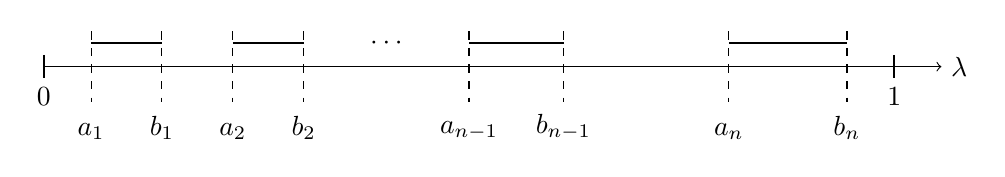
\begin{tikzpicture}[scale=3]

    % Axis
    \draw[->] (0,0) -- (3.8,0) node[right] {$\lambda$};

    % Tick marks and labels at 0 and 1
    \foreach \x/\label in {0/0, 3.6/1}
    {
        \draw[thick] (\x,0.05) -- (\x,-0.05);
        \node[below=4pt] at (\x,0) {$\label$};
    }

    % Multiple disjoint clusters
    \draw[thick] (0.2,0.1) -- (0.5,0.1); % Cluster 1
    \draw[thick] (0.8,0.1) -- (1.1,0.1); % Cluster 2
    \draw[thick] (1.8,0.1) -- (2.2,0.1); % Cluster 3
    \draw[thick] (2.9,0.1) -- (3.4,0.1); % Cluster 4

    % Dots indicating missing middle clusters
    \node at (1.45,0.1) {$\cdots$};

    % Mark points a_1, b_1, a_2, b_2, ..., a_n, b_n
    \foreach \x/\label in {
        0.2/{a_1}, 0.5/{b_1},
        0.8/{a_2}, 1.1/{b_2},
        1.8/{a_{n-1}}, 2.2/{b_{n-1}},
        2.9/{a_n}, 3.4/{b_n}
    }
    {
        \draw[thin,dashed] (\x,0.15) -- (\x,-0.15);
        \node[above] at (\x,-0.35) {$\label$};
    }

\end{tikzpicture}
    \caption{Example of an eigenvalue spectrum consisting of multiple clusters.}
    \label{fig:multiple_eigenvalue_clusters}
\end{figure}

The Chebyshev polynomials $C_p$ grow rapidly outside the interval $[-1,1]$ \cite[Section 4]{cg_sharpened_convrate_Axelsson1976}. Therefore, it can be cumbersome for a computer to evaluate the product of the $C^{(j)}_{p_j}(b_i)$ terms in the denominator of \cref{eq:chebyshev_degree_p_i}, as it might result in floating-point number overflow. Instead, we first apply \cref{eq:chebyshev_polynomial_bound} and introduce the cluster condition numbers $\kappa_i = \frac{b_i}{a_i}$, where $i$ is the index of the cluster. We can then rewrite \cref{eq:chebyshev_degree_p_i} using \cref{eq:chebyshev_polynomial_approximation} as follows
\begin{equation*}
    p_i  =  \left\lceil\ln{\frac{\epsilon_i}{2}} / \ln{\frac{\sqrt{\kappa_i} - 1}{\sqrt{\kappa_i} + 1}}\right\rceil, \\
\end{equation*}
and
\begin{align*}
    \ln{\frac{\epsilon_i}{2}} & = \ln{\frac{\epsilon}{2}} - \sum_{j=1}^{i-1} \ln{C^{(j)}_{p_j}(b_i)}. \\
\end{align*}
Let $z^{(i,j)}_1 = \frac{b_j + a_j - 2b_i}{b_j - a_j}$ and $z^{(j)}_2 = \frac{b_j + a_j}{b_j - a_j}$ then
\begin{equation*}
    \ln{C^{(j)}_{p_j}(b_i)} = \ln{C_{p_j}(z^{(i,j)}_1)} - \ln{C_{p_j}(z^{(j)}_2)}.
\end{equation*}
We have, using the approximations in \cref{eq:chebyshev_polynomial_approximation}
\begin{equation}
    \ln{C_{p_j}(z^{(i,j)}_1)} \approx p_j \ln{\left|z^{(i,j)}_1 - \sqrt{\left(z^{(i,j)}_1\right)^2 - 1}\right|} - \ln{2},
    \label{eq:chebyshev_polynomial_bound_z1}
\end{equation}
and
\begin{equation}
    \ln{C_{p_j}(z^{(j)}_2)} \approx p_j \ln{\left[z^{(j)}_2 + \sqrt{\left(z^{(j)}_2\right)^2 - 1}\right]} - \ln{2},
    \label{eq:chebyshev_polynomial_bound_z2}
\end{equation}
both of which become more accurate approximations as $z,m\rightarrow\infty$. Introducing
\begin{align*}
    \zeta^{(i,j)}_1 & = z^{(i,j)}_1 - \sqrt{\left(z^{(i,j)}_1\right)^2 - 1},         \\
    \zeta^{(j)}_2   & = z^{(j)}_2 + \sqrt{\left(z^{(j)}_2\right)^2 - 1}, \text{ and} \\
    f_i             & = \frac{\sqrt{\kappa_i} - 1}{\sqrt{\kappa_i} + 1},
\end{align*}
with $\kappa_i$ the $i^{\text{th}}$ cluster condition number, and substituting the inequalities \ref{eq:chebyshev_polynomial_bound_z1} and \ref{eq:chebyshev_polynomial_bound_z2} back into the bound for $p_i$ gives
\begin{align*}
    p_i & \leq \left\lceil\frac{\ln{\frac{\epsilon}{2}} - \sum_{j=1}^{i-1} p_j\left(\ln{\zeta^{(i,j)}_1} - \ln{\zeta^{(j)}_2} \right)}{\ln{f_i}}\right\rceil  \\
        & = \left\lceil\log_{f_i}{\frac{\epsilon}{2}} - \sum_{j=1}^{i-1} p_j\left(\log_{f_i}{\zeta^{(i,j)}_1} - \log_{f_i}{\zeta^{(j)}_2} \right)\right\rceil \\
        & = \left\lceil\log_{f_i}{\frac{\epsilon}{2}} - \sum_{j=1}^{i-1} p_j\log_{f_i}\left(\frac{\zeta^{(i,j)}_1}{\zeta^{(j)}_2}\right)\right\rceil
\end{align*}
Note that in general $f_i < 1$ and $\zeta^{(i,j)}_1 > \zeta^{(j)}_2$. Therefore, term $\log_{f_i}{\left(\frac{\zeta^{(i,j)}_1}{\zeta^{(j)}_2}\right)} < 0$. So we multiply this term by $-1$ and obtain
\begin{equation}
    p_i \leq \left\lceil\log_{f_i}{\frac{\epsilon}{2}} + \sum_{j=1}^{i-1} p_j\log_{f_i}\left(\frac{\zeta^{(j)}_2}{\zeta^{(i,j)}_1}\right)\right\rceil
    \label{eq:chebyshev_degree_p_i_explicit}
\end{equation}
Evidently, adding more clusters to the left of the interval $[a_i,b_i]$ increases the degree $p_i$ of the Chebyshev polynomial. Next to this, \cref{eq:chebyshev_degree_p_i_explicit} reduces to the classical CG iteration bound \cref{eq:cg_convergence_rate_bound_iterations} for a single cluster when $i = N_{\text{clusters}} = 1$.

Equation \ref{eq:chebyshev_degree_p_i_explicit} gives us a way to calculate the Chebyshev degree $p_i$ of the $i^{\text{th}}$ cluster $[a_i,b_i]$ in terms of the Chebyshev degrees of the previous clusters. To obtain a bound on the number of iterations for the CG method we sum the Chebyshev degrees of all the clusters
\begin{equation}
    m_{N_{\text{clusters}}} = \sum_{i=1}^{N_{\text{clusters}}} p_i
    \label{eq:cg_iteration_bound_multiple_clusters}
\end{equation}

\subsection{Multiple tail clusters}\label{sec:cg_single_eigenvalue_tail_clusters}
We have not yet generalized to an eigenvalue spectrum consisting of multiple tail clusters. Moreover, the most general eigenvalue spectrum can consist of any combination of \textit{regular} and tail clusters, as shown in \cref{fig:general_spectrum}.
\begin{figure}[H]
    \centering
    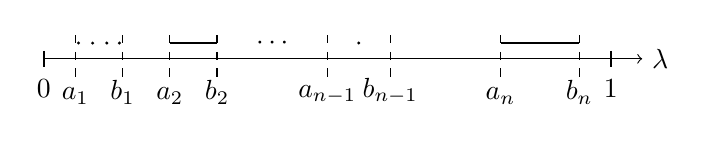
\begin{tikzpicture}[scale=2]

    % Axis
    \draw[->] (0,0) -- (3.8,0) node[right] {$\lambda$};

    % Tick marks and labels at 0 and 1
    \foreach \x/\label in {0/0, 3.6/1}
    {
        \draw[thick] (\x,0.05) -- (\x,-0.05);
        \node[below=4pt] at (\x,0) {$\label$};
    }

    % Multiple disjoint clusters
    \foreach \x in {0.22,0.31,0.40,0.48} 
        \fill (\x,0.1) circle (0.3pt); % Tail cluster
    \draw[thick] (0.8,0.1) -- (1.1,0.1); % Cluster 1
    \foreach \x in {2.0} 
        \fill (\x,0.1) circle (0.3pt); % Single eigenvalue cluster
    \draw[thick] (2.9,0.1) -- (3.4,0.1); % Cluster 2

    % Dots indicating missing middle clusters
    \node at (1.45,0.1) {$\cdots$};

    % Mark points a_1, b_1, a_2, b_2, ..., a_n, b_n
    \foreach \x/\label in {
        0.2/{a_1}, 0.5/{b_1},
        0.8/{a_2}, 1.1/{b_2},
        1.8/{a_{n-1}}, 2.2/{b_{n-1}},
        2.9/{a_n}, 3.4/{b_n}
    }
    {
        \draw[thin,dashed] (\x,0.15) -- (\x,-0.15);
        \node[above] at (\x,-0.35) {$\label$};
    }

\end{tikzpicture}
    \caption{Example of the most general eigenvalue spectrum. In order from left to right; a tail cluster $[a_1, b_1]$, a regular cluster $[a_2, b_2]$, a tail cluster $[a_{n-1}, a_{n-1}]$ with a single eigenvalue and another regular cluster $[a_n, b_n]$.}
    \label{fig:general_spectrum}
\end{figure}

Fortunately, there is a natural way to generalize the CG bound to this case. Let $\Lambda_{t}$ be the set of all eigenvalues residing in tail clusters. Now consider a polynomial similar to \cref{eq:residual_polynomial_rm} for the case $i=2$, that is
\begin{equation}
    r_{t}(x) = \prod_{\lambda\in\Lambda_{t}} \left(1 - \frac{x}{\lambda}\right).
    \label{eq:residual_polynomial_tail_clusters}
\end{equation}
The polynomial $r_t(x)$ is indeed the natural choice for polynomials of the tail clusters. To see this, suppose we were to consider separate polynomials $r_{t_j}(x)$ for each tail cluster $j$ consisting of $t_j$ tail eigenvalues $\lambda_j\in\Lambda_{t_j}$. Then we need $r_{t_j}(\lambda_j) = 0, \ \forall \lambda_j \in \Lambda_{t_j}, \ \forall j$. The most natural choice for such a polynomial is
\begin{equation}
    r_{t_j}(x) = \prod_{\lambda\in\Lambda_{t_j}} \left(1 - \frac{x}{\lambda}\right).
\end{equation}
Now, consider the global residual polynomial $r(x)$ defined as
\begin{equation}
    r(x) = \prod_{j} r_{t_j}(x) \prod_{i=1}^{N_{\text{clusters}}} C^{(i)}_{p_i}(x)= \prod_{\lambda\in\Lambda_{t}} \left(1 - \frac{x}{\lambda}\right)\prod_{i=1}^{N_{\text{clusters}}} C^{(i)}_{p_i}(x) = r_t(x)\prod_{i=1}^{N_{\text{clusters}}} C^{(i)}_{p_i}(x), 
    \label{eq:residual_polynomial_tail_clusters_global}
\end{equation}
where $\Lambda_{t} = \cup_{j} \Lambda_{t_j}$. Hence, we recover $r_t(x)$ from \cref{eq:residual_polynomial_tail_clusters} and see that is a natural generalization.

The degree of $r_{t}$ is equal to the number of eigenvalues in $\Lambda_{t}$, which we denote as $N_{t}$. Now $N_{t}$, unlike the degrees $p_i$ of the Chebyshev polynomials $C^{(i)}_{p_i}$ corresponding to the clusters, is fixed. Therefore, the contribution of the tail clusters to the CG bound is simply $N_{t}$. However, $r_{t}$ may still influence the degrees $p_i$ through its contribution to the global residual polynomial $r(x)$ defined in \cref{eq:residual_polynomial_tail_clusters_global}. In particular, we rewrite \cref{eq:chebyshev_degree_p_i_explicit} as
\begin{equation}
    p_i \leq \left\lceil\log_{f_i}{\frac{\epsilon}{2}} + \sum_{j=1}^{i-1} p_j\log_{f_i}{\frac{\zeta^{(j)}_2}{\zeta^{(i,j)}_1}} - \sum_{\lambda\in\Lambda_{t}}
    \log_{f_i}\left(1-\frac{h_i}{\lambda}\right)\right\rceil,
\end{equation}
where
\[
    h_i = \arg\max_{x\in[a_i,b_i]} \left|r_{t}(x)\right|,
\]
that is, we make the approximation that the maximum of the tail residual polynomial $r_{t}$ on the $i^{\text{th}}$ cluster is attained at one of that cluster's endpoints. For instance, in the case that the $i^{\text{th}}$ cluster lies fully to the right of all tail eigenvalues, that is $a_i > \max\{\lambda : \lambda \in \Lambda_{t}\}$, we have $h_i = b_i$. Finally, we can combine \cref{eq:chebyshev_degree_p_i_explicit}
and \cref{eq:cg_iteration_bound_multiple_clusters} as
\begin{equation}
    m_N = N_{t} + \sum_{i=1}^{N_{\text{clusters}}} p_i.
    \label{eq:cg_iteration_bound_multiple_clusters_s}
\end{equation}

\subsection{Algorithm for generalized CG bound}\label{sec:cg_multi_cluster_bound_algorithm}
We summarize the techniques outlined in this section in \cref{alg:generalized_cg_bound}. The algorithm takes a set of clusters, a (possibly empty) set of tail eigenvalues $\Lambda_t$ and a relative error tolerance $\epsilon$ as input and returns the generalized multi-tail-cluster CG iteration bound $m_N$. The algorithm iterates over all clusters, calculating the Chebyshev degree $p_i$ for each cluster based on the previous clusters' degrees and the relative error tolerance. It also treats tail eigenvalues as discussed in \cref{sec:cg_single_eigenvalue_tail_clusters}. Finally, it sums up all the Chebyshev degrees and the contribution from the tail eigenvalues to obtain the multi-cluster CG bound.
\begin{algorithm}[H]
    \caption{$\operatorname{GeneralizedCGIterationBound}(\text{clusters}, \Lambda_t, \epsilon)$}
    \begin{algorithmic}[1]
        \State \textbf{Input:} Sorted set $\text{clusters} = \langle[a_1, b_1], [a_2, b_2], \ldots, [a_{N_{\text{clusters}}}, b_{N_{\text{clusters}}}]\rangle$, a set of tail eigenvalues $\Lambda_t$ and relative error tolerance $\epsilon$
        \State \textbf{Output:} Generalized multi-tail-cluster CG iteration bound $m_N$
        \State Set $N_{t} \gets |\Lambda_{t}|$
        \State Initialize $P \gets \emptyset$
        \For{$[a_i, b_i] \in \text{clusters}$}
        \State $f_i \gets \frac{\sqrt{\kappa_i} - 1}{\sqrt{\kappa_i} + 1}$, where $\kappa_i = \frac{b_i}{a_i}$
        \State $r_{t,\text{max}} \gets \max\{\left|r_{t}(x)\right| : x \in [a_i, b_i]\}$
        \State $\epsilon_i \gets \ln(\epsilon) - \ln(r_{t,\text{max}})$
        \For{$[a_j, b_j] \in \text{clusters}_{<i}$} \Comment{$\text{clusters}_{<i}$ = all clusters to the left of $[a_i, b_i]$}
        \State $z_1 \gets \frac{b_j + a_j - 2b_i}{b_j - a_j}$
        \State $z_2 \gets \frac{b_j + a_j}{b_j - a_j}$
        \State $p_j \gets P[j]$
        \State $\epsilon_i \gets \epsilon_i - p_j \left(\ln\left(z_1 - \sqrt{z_1^2 -1}\right) - \ln\left(z_2 + \sqrt{z_2^2 -1}\right)\right)$
        \EndFor
        \State $p_i \gets \left\lceil\log_{f_i}\left(\frac{\epsilon_i}{2}\right)\right\rceil$
        \State $P \gets P \cup \langle p_i \rangle$
        \EndFor
        \State $m_{N} \gets N_{t} + \sum_{i=1}^{N_{\text{clusters}}} P[i]$
        \State \Return $m_{N}$
    \end{algorithmic}
    \label{alg:generalized_cg_bound}
\end{algorithm}

\section{Algorithms for sharpened CG iteration bounds}\label{sec:cg_iteration_bound_algorithm}
In this section we combine the findings of \cref{sec:performance_ratio,sec:tail_cluster_bound_performance,sec:multiple_clusters} to derive a flexible algorithm for determining a sharpened CG bound. The main goal of the algorithms in this section is to partition a given eigenspectrum in such a way such that the resulting set of clusters and possibly tail eigenvalues can be fed into \cref{alg:generalized_cg_bound} to obtain $m_{N_{\text{clusters}}}$. However, to ensure that $m_{N_{\text{clusters}}} < m_1$ the partitioning of the eigenspectrum should satisfy the performance conditions derived in \cref{sec:performance_threshold,sec:tail_cluster_bound_performance}. 

\subsection{Multi-cluster CG iteration bound}\label{sec:partition_eigenspectrum}
Here we only consider partitioning a spectrum into clusters, that is we do not look for possible tail eigenvalues. Later in \cref{sec:partition_eigenspectrum_tail} we will see how to extend the algorithms we derive to the incorporate clusters of tail eigenvalues. 

The idea is to use a simple algorithm to split an eigenspectrum into two clusters. Then, we calculate the left and right cluster condition numbers $\kappa_l$ and $\kappa_r$ and check if the approximate threshold condition in \cref{eq:threshold_inequality_explicit_expansion} is satisfied. In fact, the algorithm recursively applies the previous two steps, stopping only when the threshold condition is not satisfied. The result is a list of indices at which to split the eigenspectrum, yielding an ordered set of clusters $\langle[a_i, b_i]\rangle_{i=1}^{N_{\text{clusters}}}$, where $N_{\text{clusters}}$ is the number of clusters. Finally, we can use \cref{alg:generalized_cg_bound} to calculate the generalized CG iteration bound for a spectrum consisting of purely clusters, $m_{N_{\text{clusters}}}$.

To that end, suppose we are given a sorted set of eigenvalues $\sigma = \langle\lambda_1, \lambda_2, \ldots, \lambda_n\rangle$ with $0 < \lambda_1 \leq \lambda_2 \leq \cdots \leq \lambda_n$. We need to find an \textit{optimal} way of splitting this set in two disjoin sets. In order to do so we turn to \cref{fig:two_cluster_bound_performance}, in which it is shown that the performance of the two-cluster bound $m_2$ relative to the classical bound $m_1$ for fixed $\kappa$ increases both with smaller $\kappa_l$ and $\kappa_r$. Therefore, we expect to get the greatest performance gain from splitting the spectrum between those eigenvalues that share the largest ratio. That is to say, we can always write 
\[
    \kappa = \frac{\lambda_{k^*}}{\lambda_1}\frac{\lambda_{k^*+1}}{\lambda_{k^*}}\frac{\lambda_n}{\lambda_{k^*+1}} = \kappa_l\kappa_m\kappa_r,
\]
where $\kappa_l = \frac{\lambda_{k^*}}{\lambda_1}$, $\kappa_m = \frac{\lambda_{k^*+1}}{\lambda_{k^*}}$ and $\kappa_r = \frac{\lambda_n}{\lambda_{k^*+1}}$. The split index $k^*$ must be chosen such that the ratio $\frac{\lambda_{k^*+1}}{\lambda_{k^*}}$ is maximized and, simultaneously, $\kappa_l,\kappa_r$ are minimized.

Therefore, we choose to split the eigenspectrum at the \textit{largest logarithmic gap} between consecutive eigenvalues, resulting in \cref{alg:split_eigenspectrum}.
\begin{algorithm}[H]
    \caption{$\operatorname{SplitEigenspectrum}(\sigma)$}
    \begin{algorithmic}[1]
        \State \textbf{Input:} Sorted eigenvalues $\sigma = \langle\lambda_1, \lambda_2, \ldots, \lambda_n\rangle$ with $\lambda_i > 0$
        \State \textbf{Output:} Split index $k^*$ such that clusters are $\langle\lambda_1, \ldots, \lambda_{k^*}\rangle$ and $\langle\lambda_{k^*+1}, \ldots, \lambda_n\rangle$
        \State Initialize $\text{max\_gap} \gets 0$, $k^* \gets 1$
        \For{$i = 1$ to $n-1$}
        \State Compute logarithmic gap: $g_i \gets \ln(\lambda_{i+1}) - \ln(\lambda_i) = \ln\left(\frac{\lambda_{i+1}}{\lambda_i}\right)$
        \If{$g_i > \text{max\_gap}$}
        \State $\text{max\_gap} \gets g_i$
        \State $k^* \gets i$
        \EndIf
        \EndFor
        \State \Return $k^*$
    \end{algorithmic}
    \label{alg:split_eigenspectrum}
\end{algorithm}
The logarithm of the ratio of consecutive eigenvalues is used to ensure that the split index $k^*$ is chosen such that the ratio $\frac{\lambda_{k^*+1}}{\lambda_{k^*}}$ is maximized, as discussed above. The added advantage of using the logarithm instead of the ratio directly is that it prevents extremely large values in the inequality in line 6 of \cref{alg:split_eigenspectrum}, possibly causing floating-point precision issues in the evaluation of said inequality.

Recursive application of \cref{alg:split_eigenspectrum} with stopping criterion based on the threshold condition in \cref{eq:threshold_inequality_explicit_expansion} leads to \cref{alg:partition_eigenspectrum}.
\begin{algorithm}[H]
    \caption{$\operatorname{PartitionEigenspectrum}(\sigma)$}
    \begin{algorithmic}[1]
        \State \textbf{Input:} Sorted eigenvalues $\sigma = \langle\lambda_1, \lambda_2, \ldots, \lambda_n\rangle$
        \State \textbf{Output:} Sorted partition indices $K^* = \langle k^*_1, k^*_2, \ldots, k^*_{N_{\text{clusters}}-1}, n\rangle$
        \If{$\sigma = \emptyset$}
            \State \Return $\emptyset$
        \ElsIf{$|\sigma| = n \leq 2$}
            \State \Return $\langle n \rangle$
        \EndIf
        \State $\kappa \gets \frac{\lambda_n}{\lambda_1}$
        \State $k^* \gets \operatorname{SplitEigenspectrum}(\sigma)$
        \State $\kappa_l \gets \frac{\lambda_{k^*}}{\lambda_1}$
        \State $\kappa_r \gets \frac{\lambda_n}{\lambda_{k^*+1}}$
        \If{$\kappa > T^{(0)}(\kappa_l,\kappa_r)$}
        \State \Return $\operatorname{PartitionEigenspectrum}(\sigma_{\leq k^*}) \cup k^* + \operatorname{PartitionEigenspectrum}(\sigma_{>k^*})$
        \Else
        \State \Return $\langle n \rangle$ \Comment{No further partitioning needed, return last index}
        \EndIf
    \end{algorithmic}
    \label{alg:partition_eigenspectrum}
\end{algorithm}
Note that \cref{alg:partition_eigenspectrum} returns at a minimum a set containing only the last index $K^*= \langle n \rangle$, if the threshold condition is not satisfied for any split. Additionally, the value $k^*$ is added (element-wise) to the result of the right-hand recursion in line 8 of \cref{alg:partition_eigenspectrum}. This is to ensure that the resulting set of indices $K^*$ contains the correct, global indices of the eigenvalues in the spectrum, as the right-hand recursion only returns indices relative to the right-hand side of the split.

Finally, we can combine the partitioning from \cref{alg:partition_eigenspectrum} with the Chebyshev degree calculation from \cref{alg:generalized_cg_bound} to obtain the sharpened CG bound \cref{alg:multi_cluster_cg_bound}. It is important to realize that partitioning done by \cref{alg:partition_eigenspectrum} can also produce clusters consisting of a single eigenvalue, i.e. $[a_i, b_i] = [\lambda_i, \lambda_i]$. Clusters of this kind automatically satisfy the sparsity condition in \cref{eq:tail_cluster_bound_sparsity_condition} for any $\kappa\geq1$, $\kappa_l,\kappa_r<\kappa$ and $\epsilon\leq\frac{1}{2}$. Therefore, these single eigenvalue clusters belong to the set of tail eigenvalues $\Lambda_t$. Even though we did not aim to find tail eigenvalues, we are forced to accept their existence in this case. Not merely because single eigenvalue clusters satisfy the sparsity condition, but also because the Chebyshev polynomial $C^{(i)}_{p_i}$ corresponding to a single eigenvalue cluster is not well-defined.
\begin{algorithm}[H]
    \caption{$\operatorname{MultiClusterCGIterationBound}(\sigma, \epsilon)$}
    \begin{algorithmic}[1]
        \State \textbf{Input:} Sorted eigenvalues $\sigma = \langle\lambda_1, \lambda_2, \ldots, \lambda_n\rangle$, target relative error $\epsilon$
        \State \textbf{Output:} Sharpened CG iteration bound $m_{N_{\text{cluster}}} \leq m_1$
        \State Initialize $\Lambda_t \gets \emptyset$, $\text{clusters} \gets \emptyset$, $k_a \gets 1$
        \State $K^* \gets \operatorname{PartitionEigenspectrum}(\sigma)$
        \For{$k_b \in K^*$}
        \If{$k_a = k_b$}
        \State $\Lambda_t \gets \Lambda_t \cup \{\sigma[k_a]\}$ \Comment{Single eigenvalue cluster, add to tail eigenvalues}
        \State \textbf{continue} 
        \EndIf
        \State $\text{clusters} \gets \text{clusters} \cup \langle[\sigma[k_a], \sigma[k_b]]\rangle$
        \State $k_a \gets k_b + 1$
        \EndFor
        \State $m_{N_{\text{cluster}}} \gets \operatorname{GeneralizedCGIterationBound}(\text{clusters}, \Lambda_t, \epsilon)$
        \State \Return $m_{N_{\text{cluster}}}$
    \end{algorithmic}
    \label{alg:multi_cluster_cg_bound}
\end{algorithm}
Algorithm \ref{alg:multi_cluster_cg_bound} first partitions the eigenspectrum into clusters using \cref{alg:partition_eigenspectrum}. Then, it constructs a list of clusters, leaving out single eigenvalue clusters, but adding them to the list of tail eigenvalues instead. Finally, the algorithm computes the sharpened CG bound using \cref{alg:generalized_cg_bound}. In the case that the eigenspectrum is never partitioned, i.e. the threshold condition is never satisfied, the algorithm returns the classical CG bound $m_1$ from \cref{eq:cg_convergence_rate_bound_iterations}.

\subsection{Multi-tail-cluster CG iteration bound}\label{sec:partition_eigenspectrum_tail}
In this section we adapt \cref{alg:partition_eigenspectrum} to check additional conditions on $p=k^*$, that is
\[
    k^* < \left\lfloor\frac{\sqrt{\kappa_l}}{2}\ln{\frac{2}{\epsilon}} + 1 \right\rfloor
\] 
and the sparsity condition from \cref{eq:tail_cluster_bound_sparsity_condition}. This results in \cref{alg:partition_eigenspectrum_tails}. Similar to \cref{alg:partition_eigenspectrum}, the algorithm recursively partitions the eigenspectrum, returning the set of split indices $K^*$. In addition, \cref{alg:partition_eigenspectrum_tails} also updates a preinitialized set of tail eigenvalues $\Lambda_t$ and a set of tail cluster start indices $I_t$. The tail cluster start indices are initialized to an offset value, which is incremented by the size of the left-hand partition at each recursive call. This way, the tail cluster start indices are always relative to the original eigenspectrum. The use for tracking the start indices of the tail clusters is to ensure that the tail eigenvalues can be identified and left out of the set of regular clusters upon calling the generalized multi-tail-cluster CG iteration bound in \cref{alg:multi_tail_cluster_cg_bound}.
\begin{algorithm}[H]
    \caption{$\operatorname{PartitionEigenspectrumTails}(\sigma, \Lambda_t\gets\emptyset, I_t\gets\emptyset, \text{offset}\gets1)$}
    \begin{algorithmic}[1]
        \State \textbf{Input:} Sorted eigenvalues $\sigma = \langle\lambda_1, \lambda_2, \ldots, \lambda_n\rangle$, preinitialized set of tail eigenvalues $\Lambda_t$, preinitialized set of tail cluster start indices $I_t$ and an offset for the tail indices equal to 1
        \State \textbf{Output:} Sorted partition indices $K^* = \langle k^*_1, k^*_2, \ldots, k^*_{N_{\text{clusters}}-1}, n\rangle$, updated set of tail eigenvalues $\Lambda_t$ and updated set of tail cluster start indices $I_t$
        \If{$\sigma = \emptyset$}
            \State \Return $\emptyset$
        \ElsIf{$|\sigma| = n = 1$}
            \State $\Lambda_t \gets \Lambda_t \cup \{\lambda_1\}$ 
            \State $I_t \gets I_t \cup \{\text{offset}\}$
            \State \Return $\langle 1 \rangle$
        \EndIf
        \State $\kappa \gets \frac{\lambda_n}{\lambda_1}$
        \State $k^* \gets \operatorname{SplitEigenspectrum}(\sigma)$
        \State $\kappa_l \gets \frac{\lambda_{k^*}}{\lambda_1}$
        \State $\kappa_r \gets \frac{\lambda_n}{\lambda_{k^*+1}}$
        \If{$k^* < \left\lfloor\frac{\sqrt{\kappa_l}}{2}\ln{\frac{2}{\epsilon}} + 1 \right\rfloor$ and $k^* \leq \left\lfloor\sqrt{\frac{\kappa}{\kappa_r}}\log_{\frac{4\kappa}{\kappa_l}}\left(\frac{2}{\epsilon}\right)\right\rfloor$}
            \State $\Lambda_t \gets \Lambda_t \cup \sigma_{\leq k^*}$ 
            \State $I_t \gets I_t \cup \{\text{offset}\}$
            \State \Return $\langle k^* \rangle \cup k^* + \operatorname{PartitionEigenspectrumTails}(\sigma_{>k^*}, \Lambda_t, I_t, \text{offset} + k^*)$
        \ElsIf{$\kappa > T^{(0)}(\kappa_l,\kappa_r)$}
            \State \Return \begin{varwidth}[t]{\linewidth}
                $\operatorname{PartitionEigenspectrumTails}(\sigma_{\leq k^*}, \Lambda_t, I_t, \text{offset}) \cup \dots$\par
                $k^* + \operatorname{PartitionEigenspectrumTails}(\sigma_{>k^*}, \Lambda_t, I_t, \text{offset} + k^*)$
            \end{varwidth}
        \Else
            \State \Return $\langle n \rangle$ \Comment{No further partitioning needed, return last index}
        \EndIf
    \end{algorithmic}
    \label{alg:partition_eigenspectrum_tails}
\end{algorithm}

We are now in a position to formulate the final algorithm of this chapter, the multi-tail-cluster CG iteration bound \cref{alg:multi_tail_cluster_cg_bound}.
\begin{algorithm}[H]
    \caption{$\operatorname{MultiTailClusterCGIterationBound}(\sigma, \epsilon)$}
    \begin{algorithmic}[1]
        \State \textbf{Input:} Sorted eigenvalues $\sigma = \langle\lambda_1, \lambda_2, \ldots, \lambda_n\rangle$, target relative error $\epsilon$
        \State \textbf{Output:} Multi-tail-cluster CG iteration bound $m_{N_{\text{tail-cluster}}} \leq m_1$
        \State Initialize $\Lambda_t \gets \emptyset$, $I_t\gets\emptyset$, $\text{clusters} \gets \emptyset$, $k_a\gets 1$
        \State $K^* \gets \operatorname{PartitionEigenspectrumTails}(\sigma, \Lambda_t, I_t)$
        \For{$k_b \in K^*$}
        \If{$k_a \in I_t$}
            \State \textbf{continue} \Comment{Skip tail clusters, they are already added to $\Lambda_t$}
        \EndIf
        \State $\text{clusters} \gets \text{clusters} \cup \langle[\sigma[k_a], \sigma[k_b]]\rangle$
        \State $k_a \gets k_b + 1$
        \EndFor
        \State $m_{N_{\text{tail-cluster}}} \gets \operatorname{GeneralizedCGIterationBound}(\text{clusters}, \Lambda_t, \epsilon)$
        \State \Return $m_{N_{\text{tail-cluster}}}$
    \end{algorithmic}
    \label{alg:multi_tail_cluster_cg_bound}
\end{algorithm}